\subsection{Architecture Feasibility}
This chapter uses the same cycle-level accurate simulator with over a decade of development in industry from the previous chapter.
The architecture and core fusion mechanics are similar to the work described in~\cite{kim2007tflex,putnam2010e2}.
To ensure the accuracy of the simulator it is validated against an RTL implementation of the processor.
This validation is done by running workloads on RTL either in simulation or an FPGA and comparing the traces cycle by cycle with the software simulator.
Parts of the fusion mechanism have been modeled in RTL, allowing us to also validate it.
Due to the fact that the architecture uses the EDGE ISA~\cite{smith2006edge} McPAT cannot be used to model power consumption as EDGE differs from traditional CISC/RISC cores that are modeled in McPAT.
Instead a coarse grained power model is used, either a core is turned on or or it is off. 


\begin{figure}[t]
    \centering
	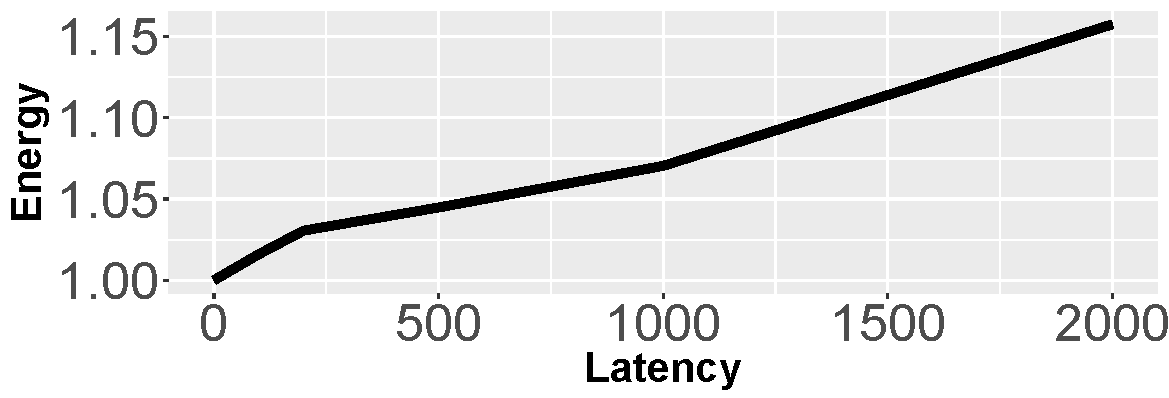
\includegraphics[width=0.4\textwidth]{cases-paper/graphics/Exploration/lat_en_2000.pdf}
\vspace*{-5mm}
    \caption{Relative increase in energy consumption when increasing the reconfiguration latency. Baseline is 0 cycle latency.}
    \label{fig:enlatency}
\end{figure}
\subsection{Fusing Cores}
In this processor, the micro-architecture is distributed: register files, Load Store Queues (LSQs), L1 caches and ALUs all look like nodes on a network.
This means that when cores are fused together, this is similar to adding an extra node to the network.
When cores are fused, one of the cores will be executing a non-speculative block from a single thread whilst all other cores excute speculative blocks that are predicted from the same thread.
A simple round robin policy is used to choose which core is going to execute a speculative block.
Whenever the blocks are committed the processor also pick a new core to execute the next non-speculative block.
When a new thread is started on a fused core the OS and runtime write the new core mapping to a system register.
The hardware then flushes these cores if they are not idle and sets the PC of the first block of that thread on one core in the core fusion and starts executing.
Fusing cores is therefore a lightweight process.
Figure~\ref{fig:enlatency} shows how the reconfiguration latency will affect the average energy consumption of each of the SD-VBS benchmarks, this is relative to the energy consumption when the latency is set to 0 cycles.
As can be seen, increasing the latency up to 2000 cycles, a 20x increase in latency, only affects it by 15\%.
%Fusing cores is a lightweight process
%
%Fusing cores is a lightweight process.
%The uarch is distributed and the register file, LSQ/L1 cache and ALUs look like nodes on a network.
%Adding more cores is similar to adding more nodes. In a group of fused cores, one core is running the non-speculative block from a single thread and the others are running speculative blocks from the same thread that are predicted.
%A simple round robin policy is used to pick the next core to run a block.
%As blocks commit the core running the non-speculative block moves.
%To start a thread on a fused core, the OS, runtime, application writes the new core mapping to a system register, then the hw flushes these cores if they are not idle, sets the PC of the first block on one core and starts executing. 
%
%The simulator has almost a decade of development and is a cycle-level full system simulator that boots the Linux kernel.
% It’s validated by running workloads on RTL (either in simulation or on an FPGA) and comparing the traces cycle by cycle between the hardware and the simulator.
% Fusion studies are done in simulation because the RTL does not implement core fusion currently and we are trying to learn what the right uarch. 
%Parts of fusion have been modeled in RTL and results match what we see in simulation.
%
% We use a course grained power model -- either the core is on or the core is off. 
%A model such as McPAT is not useful for this uarch because the activation factors are too different from traditional CISC/RISC cores that McPAT models. 
%The main focus of the work though is not on the power gains but on effectively utilizing DMPs.
